\documentclass[12pt]{article}
\usepackage[top=2cm,bottom=2.5cm,left=2cm,right=2cm,marginparwidth=2cm]{geometry}
%% Language and font encodings
\usepackage[english]{babel}
\usepackage[utf8x]{inputenc}
\usepackage{listings}
\usepackage{minted}
\usepackage[shortlabels]{enumitem}

%% Sets page size and margins

\usepackage{float}
%% Useful packages
% \usepackage{amsmath}
\usepackage{amsmath,amssymb,amsthm,bm}
\usepackage[colorinlistoftodos]{todonotes}
\usepackage[colorlinks=true, allcolors=blue]{hyperref}
\usepackage{listings}
\usepackage{url}
\usepackage{graphicx}
\graphicspath{ {./images/} }
% \DeclareGraphicsExtensions{.pdf,.jpg,.png}

\newtheoremstyle{quest}{\topsep}{\topsep}{}{}{\bfseries}{}{ }{\thmname{#1}\thmnote{ #3}.}
\theoremstyle{quest}
\newtheorem*{problem}{Problem}
\newenvironment{solution}
  {\begin{proof}[Solution]}
  {\end{proof}}
  
 \DeclareMathOperator{\diag}{diag}


%% defined colors
\definecolor{Blue}{rgb}{0,0,0.5}
\definecolor{Green}{rgb}{0,0.75,0.0}
\definecolor{LightGray}{rgb}{0.6,0.6,0.6}
\definecolor{DarkGray}{rgb}{0.3,0.3,0.3}

\title{CMPSC 448: Machine Learning and AI \\ Homework 5}
\author{}
\date{}

\begin{document}
\maketitle

\section*{Instruction}
This HW includes both theory and implementation problems. Please note,
\begin{itemize}
    \item Your code must work with Python 3.7+
    \item You need to submit a report in PDF including all written deliverable, and all implementation codes so one could regenerate your results.
    \item For programming part of PCA problem, you can import any module you would like from \textsf{scikit-learn} or other external libraries to minimize the amount of implementation required to get the coding problem done. Submit your code in \textsf{Problem.py}.
\end{itemize}

\section*{PCA}
\begin{problem}[1] [20 points]
As we discussed in the lecture, the PCA algorithm is sensitive to scaling and pre-processing of data. In this problem, we explore few data pre-processing operations on data matrices.

\begin{enumerate}
    \item Explain what does each of the following data processing operation mean, why it is important, and how you apply to a data matrix $\bm{X} \in \mathbb{R}^{n \times d}$, $n$ samples each with $d$ features \footnote{For an implementation of these operation in \textsf{scikit-learn} please see \href{https://scikit-learn.org/stable/modules/preprocessing.html}{this}.} (if it helps, use mathematical equations to show the calculations).
    \begin{enumerate}
        \item Centering or mean removal
        \item Scaling of a feature to a range $[a, b]$
        \item Standardization
        \item Normalization (between 0 and 1)
    \end{enumerate}
    \item Apply the above operations to the following data matrix with 5 samples and two features independently and show the processed data matrix. For scaling pick $a = 0$ and $b = 1$.
        \begin{equation*}
            \bm{X} = \begin{bmatrix}
            1 & 2\\
            -1 & 1\\
            0 & 1\\
            2 & 4\\
            3 & 1\\
            \end{bmatrix}
        \end{equation*}
\end{enumerate}
\end{problem}

\begin{problem}[2] [20 points]
In this assignment, you will explore PCA as a technique for discerning whether low-dimensional structure exists in a set of data and for finding good representations of the data in that subspace. To this end, you will do PCA on a Iris dataset which can be loaded in \textsf{scikit-learn} using following commands:
\end{problem}

\begin{minted}{python}
from sklearn.datasets import load_iris iris = load_iris()
X = iris.data
y = iris.target
\end{minted}

\begin{enumerate}
    \item Carry out a principal component analysis on the entire \textbf{raw} dataset (4-dimensional instances) for $k = 1, 2, 3, 4$ components. How much of variance in data can be explained by the first principal component? How does the fraction of variation explained in data vary as $k$ varies?
    \item Apply the preprocessing operations from Problem 1 on raw data set and repeat part (1) on processed data. Explain any differences you observe compared to part (1) and justify.
    \item Project the raw four dimensional data down to a two dimensional subspace generated by first two top principle components (PCs) from part (2) and produce a scatter plot of the data. Make sure you plot each of the three classes differently (using color or different markers). Can you see the three Iris flower clusters?
    \item Either use your k-means++ implementation from previous homework or from \textsf{scikit-learn} to cluster data from part (3) into three clusters. Explain your observations.
\end{enumerate}

\section*{Matrix Factorization}
\begin{problem}[3] [30 points]
Recall the following objective for extracting latent features from a partially observed rating matrix via matrix factorization (MF) for making recommendations, discussed in the class:
\begin{equation}
\label{eq:matrix_fac}
  \min_{\bm{U},\bm{V}}\left[f(\bm{U},\bm{V}) \equiv \sum_{(i,j)\in\Omega}(r_{i,j}-\bm{u}_i^{\top}\bm{v}_j)^2 + \alpha\sum_{i=1}^{n}\lVert\bm{u}_i\rVert_2^2 + \beta\sum_{j=1}^{m}\lVert\bm{v}_j\rVert_2^2 \right]  
\end{equation}
where
\begin{itemize}
    \item $n$: number of users 
    \item $m$: number of items
    \item $r_{i,j}$: $(i,j)$-th element in $\bm{R} \in \mathbb{R}^{n \times m}$ input partially observed rating matrix
    \item $\Omega \subseteq [n]\times[m]$: index of observed entries in rating matrix, where $[n]$ denotes the sequence of numbers $\{1,2,\dots,n\}$.
    \item $k$: number of latent features
    \item $\bm{U} \in \mathbb{R}^{n \times k}$: the (unknown) matrix of latent feature vectors for $n$ users (the $i$th row $\bm{u}_i \in \mathbb{R}^{k}$ is the latent features for $i$th user)
    \item $\bm{V} \in \mathbb{R}^{m \times k}$: the (unknown) matrix of latent feature vectors for $m$ items (the $j$th row $\bm{v}_j \in \mathbb{R}^{k}$ is the latent features for $j$th movie)
\end{itemize}

Please do the followings:
\begin{enumerate}
    \item In solving Equation~\ref{eq:matrix_fac} with iterative Alternating Minimization algorithm (fixing $\bm{V}^{(t)}$ and taking gradient step for $\bm{U}^{(t)}$ and vice versa), discuss what happens if $\bm{U}^{(0)}$ and $\bm{V}^{(0)}$ are initialized to zero?
    \item Discuss why when there is no regularization in basic MF formulated in Equation~\ref{eq:matrix_fac}, i.e., $\alpha = \beta = 0$, each user must have rated at least $k$ movies, and each movie must have been rated by at least $k$ users (Hint: consider the closed form solution for $\bm{u}_i$ and $\bm{v}_j$ in notes and argue why these conditions are necessary without regularization).
    \item Computing the closed form solution in part (2) could be computational burden for large number of users or movies. A remedy for this would be using iterative optimization algorithms such as Stochastic Gradient Descent (SGD) where you sample movies in updating the latent features for users and sample users in updating the latent features of movies. Derive the updating rules for $\bm{u}_i^{(t)}$ and $\bm{v}_j^{(t)}$ at $t$th iteration of SGD. Show the detailed steps.
\end{enumerate}
\end{problem}

\section*{Reinforcement Learning}
\begin{figure}[ht!]
\centering
   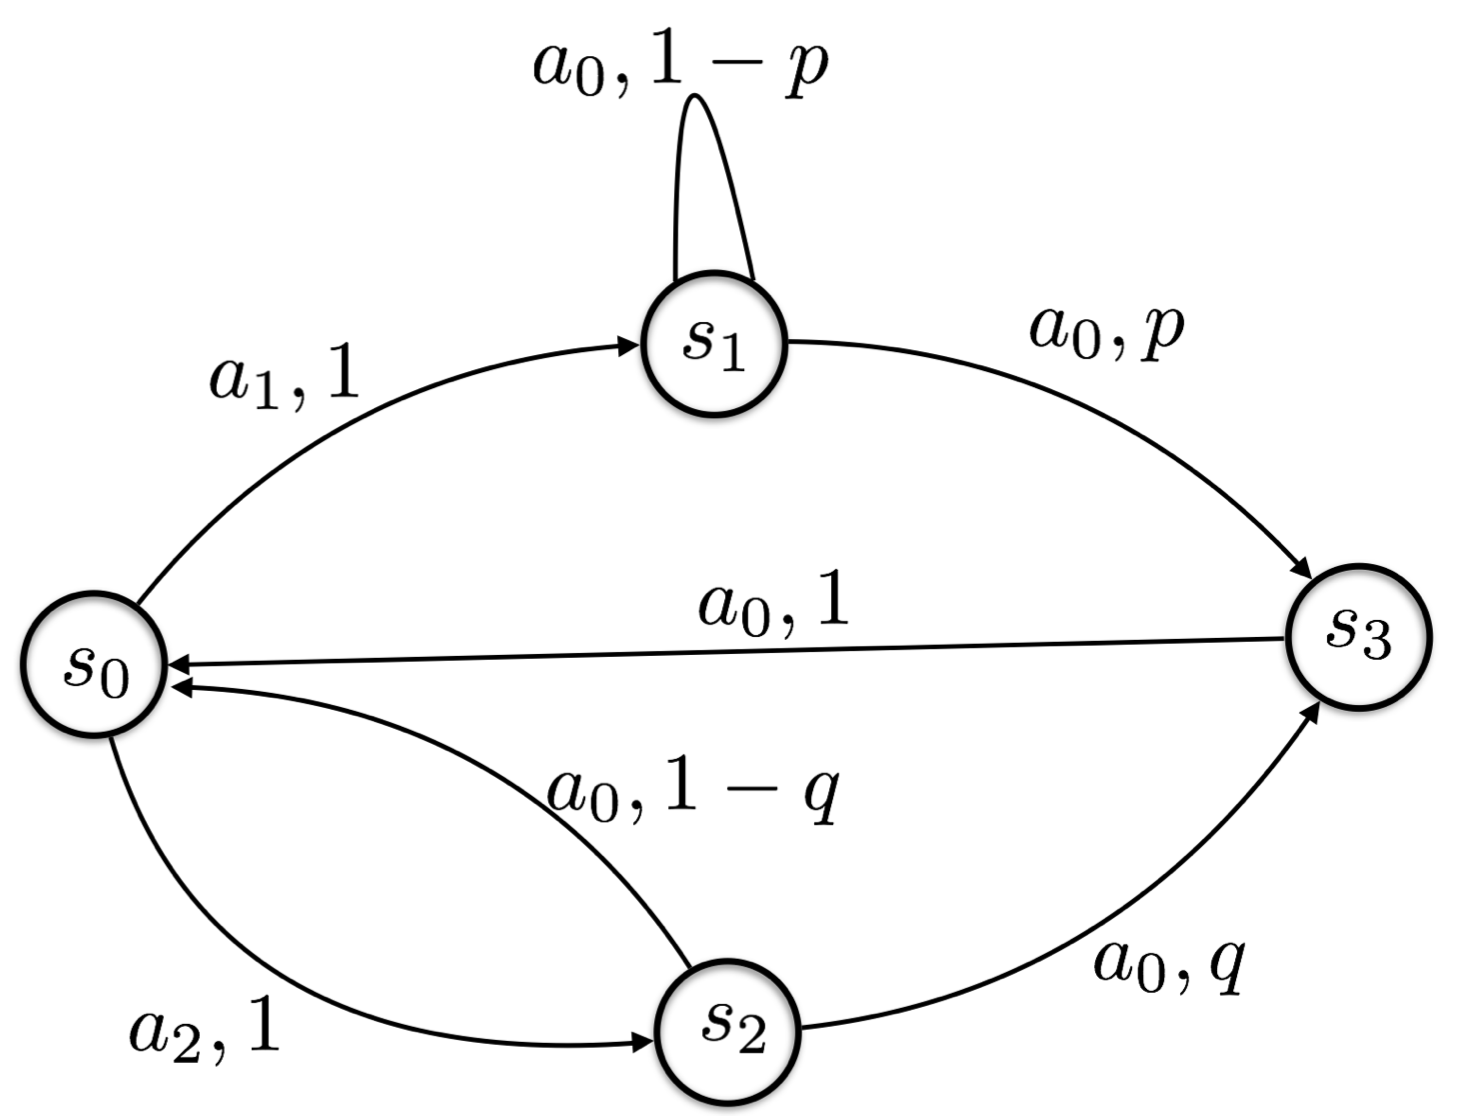
\includegraphics[width=0.5\textwidth]{mdp.png}
   \caption{A MDP with states $\mathcal{S}=\{s_0,s_1,s_2,s_3\}$ and actions $\mathcal{A}=\{a_0,a_1,a_2\}$. The reward is 10 for state $s_3$, 1 for state $s_2$, and 0 otherwise.}
   \label{fig:mdp}
\end{figure}

\begin{problem}[4] [20 points] Consider the MDP represented by a graph in Figure~\ref{fig:mdp} with discount factor $\gamma \in [0, 1)$. States are represented by circles. The pair on the arrows shows the action to be taken and the transition probability from a state to another state, respectively (please note that the representation of MDP as a graph here is slightly different from Example 3.3 in the book). Each of the parameters $p$ and $q$ are in the interval $[0, 1]$. The reward is 10 for state $s_3$, 1 for state $s_2$, and 0 otherwise. Note that this means, from $s_0$, after taking an action, it will receive 0 reward no matter what the action is. This is similar for other states. 
\begin{enumerate}
    \item List all two deterministic policies (for each state, choose an action with probability 1) for MDP in Figure~\ref{fig:mdp} starting from the initial state $s_0$ and ending at state $s_3$. For each policy $\pi$ compute the value of each state, $v_{\pi}(s_0)$, $v_{\pi}(s_1)$, $v_{\pi}(s_2)$, and $v_{\pi}(s_3)$ for $\gamma = 0$ and $p = q = \frac{1}{2}$.
    \item Show the equation representing the optimal value function for each state, i.e. $v_{\ast}(s_0)$, $v_{\ast}(s_1)$, $v_{\ast}(s_2)$, and $v_{\ast}(s_3)$. Please note the value of states will be a function of parameters $p$, $q$, and $\gamma$.
    % \item Is there a value for $p$ such that for all $\gamma \in [0,1)$ and $q \in [0,1]$, $\pi_{\ast}(s_0)=a_2$?
    \item Using $p = q = 0.25$ and $\gamma = 0.9$, compute $\pi_{\ast}$ and $v_{\ast}$ for all states of MDP. You can either solve the recursion of part (2) or implement value iteration (if you intend to do the latter, consider the approximation error $\epsilon = 10^{−3}$ as stopping criteria).
\end{enumerate}

\end{problem}

\begin{problem}[5] [10 points]
Suppose action selection is greedy. Is Q-learning then exactly the same algorithm as Sarsa? Will they make exactly the same action selections and weight updates?
\end{problem}

\end{document}